% Generated 2021-08-25 18:02:25 +0530
\subsection{Files} \label{sec:Files}


This section provides the semantic information for the \block{File} model.

\begin{figure}[ht]
  \centering
    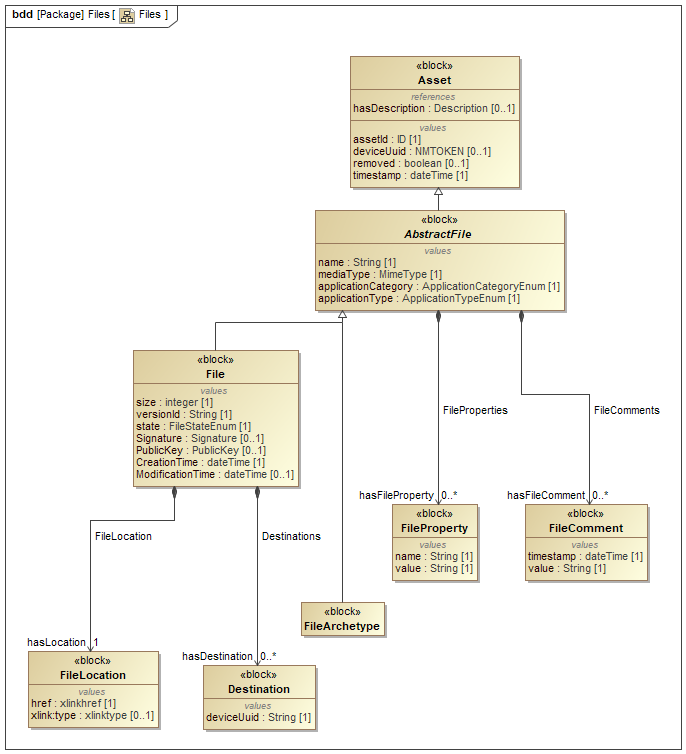
\includegraphics[width=1.0\textwidth]{figures/Files.png}
  \caption{Files Diagram}
  \label{fig:Files Diagram}
\end{figure}

\FloatBarrier


Note: See \sect{File Schema Diagrams} for XML schema.



\subsubsection{AbstractFile}
\label{sec:AbstractFile}



An \block{AbstractFile} is an abstract \block{Asset} type model that contains the common properties of the \block{File} and \block{FileArchetype} types.


\paragraph{Attributes of AbstractFile}\mbox{}
\label{sec:Attributes of AbstractFile}

\tbl{Attributes of AbstractFile} lists the attributes of \texttt{AbstractFile}.

\begin{table}[ht]
\centering 
  \caption{Attributes of AbstractFile}
  \label{table:Attributes of AbstractFile}
\tabulinesep=3pt
\begin{tabu} to 6in {|l|l|l|} \everyrow{\hline}
\hline
\rowfont\bfseries {Attribute} & {Type} & {Multiplicity} \\
\tabucline[1.5pt]{}

\property{mediaType}[AbstractFile] & \texttt{string} & 1 \\
\property{applicationCategory}[AbstractFile] & \texttt{ApplicationCategoryEnum} & 1 \\
\property{applicationType}[AbstractFile] & \texttt{ApplicationTypeEnum} & 1 \\
\end{tabu}
\end{table}
\FloatBarrier

Descriptions for attributes of \block{AbstractFile}:

\begin{itemize}

\item \property{mediaType}[AbstractFile] \newline The mime type of the file.


\item \property{applicationCategory}[AbstractFile] \newline The category of application that will use this file.

\texttt{ApplicationCategoryEnum} Enumeration:

\begin{itemize}
\item \texttt{ASSEMBLY} \newline Files regarding the fully assembled product. 
\item \texttt{DEVICE} \newline Device related files. 
\item \texttt{HANDLING} \newline Files relating to the handling of material. 
\item \texttt{MAINTENANCE} \newline File relating to equipment maintenance. 
\item \texttt{PART} \newline Files relating to a part.
 
\item \texttt{PROCESS} \newline Files related to the manufacturing process. 
\item \texttt{INSPECTION} \newline Files related to the quality inspection. 
\item \texttt{SETUP} \newline Files related to the setup of a process. 
\end{itemize}


\item \property{applicationType}[AbstractFile] \newline The type of application that will use this file.

\texttt{ApplicationTypeEnum} Enumeration:

\begin{itemize}
\item \texttt{DESIGN} \newline Computer aided design files or drawings.
 
\item \texttt{DATA} \newline Generic data. 
\item \texttt{DOCUMENTATION} \newline Documentation regarding a category of file. 
\item \texttt{INSTRUCTIONS} \newline User instructions regarding the execution of a task.
 
\item \texttt{LOG} \newline The data related to the history of a machine or process. 
\item \texttt{PRODUCTION\textunderscore PROGRAM} \newline Machine instructions to perform a process.
 
\end{itemize}

\end{itemize}


\paragraph{Elements of AbstractFile}\mbox{}
\label{sec:Elements of AbstractFile}

\tbl{Elements of AbstractFile} lists the elements of \texttt{AbstractFile}.

\begin{table}[ht]
\centering 
  \caption{Elements of AbstractFile}
  \label{table:Elements of AbstractFile}
\tabulinesep=3pt
\begin{tabu} to 6in {|l|l|} \everyrow{\hline}
\hline
\rowfont\bfseries {Element} & {Multiplicity} \\
\tabucline[1.5pt]{}
\texttt{FileProperty} (organized by \block{FileProperties}) & 0..* \\
\texttt{FileComment} (organized by \block{FileComments}) & 0..* \\
\end{tabu}
\end{table}
\FloatBarrier


Descriptions for elements of \block{AbstractFile}:

\begin{itemize}

\item \block{FileProperties} \newline \texttt{FileProperties} \glspl{organize} one or more \block{FileProperty} entities for \block{File}s.


\item \block{FileComments} \newline \texttt{FileComments} \glspl{organize} one or more \block{FileComment} entities for \block{File}s.

\end{itemize}



\subsubsection{File}
\label{sec:File}



The \block{File} \block{Asset} is an \block{AbstractFile} with information about the \block{File} instance and its \gls{URL}.


\paragraph{Attributes of File}\mbox{}
\label{sec:Attributes of File}

\tbl{Attributes of File} lists the attributes of \texttt{File}.

\begin{table}[ht]
\centering 
  \caption{Attributes of File}
  \label{table:Attributes of File}
\tabulinesep=3pt
\begin{tabu} to 6in {|l|l|l|} \everyrow{\hline}
\hline
\rowfont\bfseries {Attribute} & {Type} & {Multiplicity} \\
\tabucline[1.5pt]{}

\property{size}[File] & \texttt{integer} & 1 \\
\property{state}[File] & \texttt{FileStateEnum} & 1 \\
\end{tabu}
\end{table}
\FloatBarrier

Descriptions for attributes of \block{File}:

\begin{itemize}

\item \property{size}[File] \newline The size of the file in bytes.

\item \property{state}[File] \newline The state of the file. 

\texttt{FileStateEnum} Enumeration:

\begin{itemize}
\item \texttt{EXPERIMENTAL} \newline Used for processes other than production or otherwise defined. 
\item \texttt{PRODUCTION} \newline Used for production processes.
 
\item \texttt{REVISION} \newline The content is modified from \texttt{PRODUCTION} or \texttt{EXPERIMENTAL}.
 
\end{itemize}

\end{itemize}


\paragraph{Elements of File}\mbox{}
\label{sec:Elements of File}

\tbl{Elements of File} lists the elements of \texttt{File}.

\begin{table}[ht]
\centering 
  \caption{Elements of File}
  \label{table:Elements of File}
\tabulinesep=3pt
\begin{tabu} to 6in {|l|l|} \everyrow{\hline}
\hline
\rowfont\bfseries {Element} & {Multiplicity} \\
\tabucline[1.5pt]{}
\texttt{Signature} & 0..1 \\
\texttt{PublicKey} & 0..1 \\
\texttt{CreationTime} & 1 \\
\texttt{ModificationTime} & 0..1 \\
\texttt{FileLocation} & 1 \\
\texttt{Destination} (organized by \block{Destinations}) & 0..* \\
\end{tabu}
\end{table}
\FloatBarrier


Descriptions for elements of \block{File}:

\begin{itemize}

\item \block{Signature} \newline A secure hash of the file.

The value for \property{Signature} \textbf{MUST} be an x509 data block.

The value of \block{Signature} \MUST be \texttt{string}.

\item \block{PublicKey} \newline The public key used to verify the signature.

The value for \property{PublicKey} \textbf{MUST} be an x509 data block.

The value of \block{PublicKey} \MUST be \texttt{string}.

\item \block{CreationTime} \newline The time the file was created.

The value of \block{CreationTime} \MUST be \texttt{dateTime}.

\item \block{ModificationTime} \newline The time the file was modified.

The value of \block{ModificationTime} \MUST be \texttt{dateTime}.

\item \block{FileLocation} \newline The \gls{URL} reference to the file location. 

\item \block{Destinations} \newline \texttt{Destinations} \glspl{organize} one or more \block{Destination} elements.
\end{itemize}



\subsubsection{FileArchetype}
\label{sec:FileArchetype}



\block{FileArchetype} \block{Asset} is an \block{AbstractFile} providing information common to all versions of a file.




\subsubsection{FileProperty}
\label{sec:FileProperty}



A key-value pair providing additional metadata about a \block{File}.



\subsubsection{FileComment}
\label{sec:FileComment}



A remark or interpretation for human interpretation associated with a \block{File} or \block{FileArchetype}.


\paragraph{Attributes of FileComment}\mbox{}
\label{sec:Attributes of FileComment}

\tbl{Attributes of FileComment} lists the attributes of \texttt{FileComment}.

\begin{table}[ht]
\centering 
  \caption{Attributes of FileComment}
  \label{table:Attributes of FileComment}
\tabulinesep=3pt
\begin{tabu} to 6in {|l|l|l|} \everyrow{\hline}
\hline
\rowfont\bfseries {Attribute} & {Type} & {Multiplicity} \\
\tabucline[1.5pt]{}

\property{timestamp}[FileComment] & \texttt{dateTime} & 1 \\
\end{tabu}
\end{table}
\FloatBarrier

Descriptions for attributes of \block{FileComment}:

\begin{itemize}

\item \property{timestamp}[FileComment] \newline The time the comment was made.
\end{itemize}



\subsubsection{FileLocation}
\label{sec:FileLocation}



The \gls{URL} reference to the file location. 


\paragraph{Attributes of FileLocation}\mbox{}
\label{sec:Attributes of FileLocation}

\tbl{Attributes of FileLocation} lists the attributes of \texttt{FileLocation}.

\begin{table}[ht]
\centering 
  \caption{Attributes of FileLocation}
  \label{table:Attributes of FileLocation}
\tabulinesep=3pt
\begin{tabu} to 6in {|l|l|l|} \everyrow{\hline}
\hline
\rowfont\bfseries {Attribute} & {Type} & {Multiplicity} \\
\tabucline[1.5pt]{}

\property{href}[FileLocation] & \texttt{xlinkhref} & 1 \\
\property{xlink:type}[FileLocation] & \texttt{xlinktype} & 0..1 \\
\end{tabu}
\end{table}
\FloatBarrier

Descriptions for attributes of \block{FileLocation}:

\begin{itemize}

\item \property{href}[FileLocation] \newline A \gls{URL} reference to the file.

\texttt{href} is of type \texttt{xlink:href} from the W3C XLink specification.


\item \property{xlink:type}[FileLocation] \newline The type of href for the xlink href type. 

\textbf{MUST} be \texttt{locator} referring to a \gls{URL}
.
\end{itemize}



\subsubsection{Destination}
\label{sec:Destination}



The \block{Destination} is a reference to the target \block{Device} for this \block{File}.



\paragraph{Attributes of Destination}\mbox{}
\label{sec:Attributes of Destination}

\tbl{Attributes of Destination} lists the attributes of \texttt{Destination}.

\begin{table}[ht]
\centering 
  \caption{Attributes of Destination}
  \label{table:Attributes of Destination}
\tabulinesep=3pt
\begin{tabu} to 6in {|l|l|l|} \everyrow{\hline}
\hline
\rowfont\bfseries {Attribute} & {Type} & {Multiplicity} \\
\tabucline[1.5pt]{}

\property{deviceUuid}[Destination] & \texttt{IDREF} & 1 \\
\end{tabu}
\end{table}
\FloatBarrier

Descriptions for attributes of \block{Destination}:

\begin{itemize}

\item \property{deviceUuid}[Destination] \newline \texttt{uuid} of the target device or application.
\end{itemize}


